%%%%%%%%%%%%%%%%%%%%%%%%%%%%%%%%%%
% EL/EEE D1 Report Template
% University of Southampton
%
% author : Rhys Thomas (rt8g15)
%
% edited : 2016-11-14
%%%%%%%%%%%%%%%%%%%%%%%%%%%%%%%%%%

\documentclass[a4paper,11pt]{article}

%%%%%%%%%%%%%%%%%%%%%%%%%%%%%%%%%%
% PACKAGES
%%%%%%%%%%%%%%%%%%%%%%%%%%%%%%%%%%
\usepackage[margin=1in]{geometry}
\renewcommand{\baselinestretch}{1.2} % line spacing
\usepackage{listings}
\usepackage{color}
\usepackage{siunitx}
\usepackage{graphicx}
\usepackage{epstopdf}

\definecolor{dkgreen}{rgb}{0,0.6,0}
\definecolor{gray}{rgb}{0.5,0.5,0.5}
\definecolor{mauve}{rgb}{0.58,0,0.82}

\lstset{frame=tb,
  language=Verilog,
  aboveskip=3mm,
  belowskip=3mm,
  showstringspaces=false,
  columns=flexible,
  basicstyle={\small\ttfamily},
  numbers=none,
  numberstyle=\tiny\color{gray},
  keywordstyle=\color{blue},
  commentstyle=\color{dkgreen},
  stringstyle=\color{mauve},
  breaklines=true,
  breakatwhitespace=true,
  tabsize=3
}

%%%%%%%%%%%%%%%%%%%%%%%%%%%%%%%%%%
% DOCUMENT BEGIN
%%%%%%%%%%%%%%%%%%%%%%%%%%%%%%%%%%
\begin{document}
  
\begin{center}
{\Large{\textbf{ELEC2221 D1 -- Design and test of a sequential multiplier}}} \\ [\baselineskip]
Maciej Romanski \\
mr12g15 \\
Electronic Engineering with Computer Systems \\
Dr. Yoshishige Tsuchiya \\
Lab Group E \\
Lab completed on 2016-11-21
\end{center}

\begin{abstract}
Using SystemVerilog, the individual elements of a 4 bit (and eventually an 8-bit) hardware multiplier were written for synthesis on to a MachXO2 Pico FPGA. The modules included a 4 bit adder, 9 bit register, and a sequencer that implemented the shift and add multiplication algorithm. The code was mostly tested using Icarus Verilog, and then additional changes in the lab were tested using ModelSim. The modules were synthesised by Synplify Pro, and the FPGA was programmed using Lattice Diamond. The end result was a device that would multiply two hardcoded 8 bit numbers, displaying the 16 bit result in binary on an array of 16 LEDs.
\end{abstract}

\section{Adder design, simulation and synthesis}
The code used to implement the adder was mostly the same as the model code provided; only a few variables were changed, as well as the array sizes when scaling up to 8 bits.

\subsection{Adder simulation}
\lstset{caption={Adder testbench (adder\_tb.sv)}, label=ls:addertb}
\begin{lstlisting}
`timescale 1ns/1ps
module adder_tb;
    logic[7:0] a;
    logic[7:0] m;
    logic[7:0] sum;
    logic carry;
    logic[16:0] correct_sum;
    logic correct_carry;
    int loopa;
    int loopm;
    
    // Instantiating adder module
    adder r(.*); 
    
    initial
    begin
        a = 0;
        m = 0;
    end
    
    // For generating waveforms
    initial
    begin
        $dumpfile("adder_tb.vcd");
        $dumpvars(0, a, m, sum, carry);
    end
    
    // Loop that tests every single possible set of inputs.
    always begin
        for (loopa = 0; loopa <= 255; loopa++) begin
            for (loopm = 0; loopm <= 255; loopm++) begin
                correct_sum = loopa + loopm;
                if (correct_sum > 255)
                    correct_carry = 1;
                else
                    correct_carry = 0;                    
                $display("%d + %d = %d carry %d", a, m, sum, carry);
                // Checking to make sure that the adder module is generating the correct values.
                // 8 bit output, hence the sum is being checked against the lower 8 bits of correct_sum
                if ((sum != correct_sum[7:0]) || (carry != correct_carry))
                    $fatal;
                m++;
                #1; // Delays required by Icarus Verilog for some reason
            end
            a++;
            #1;
        end        
        $display("Test passed!");
        $finish;
    end
endmodule
\end{lstlisting}

\begin{figure}
    \centering
        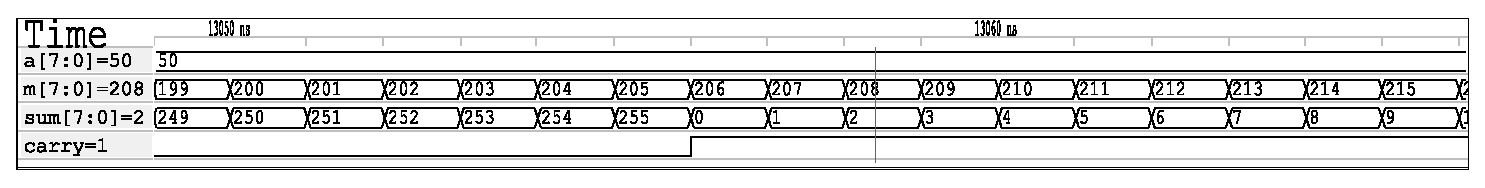
\includegraphics[scale=0.65]{../out/adder_tb.eps}
    \caption{Output waveform of the adder testbench from \SI{13049}{\nano\second} to \SI{13066}{\nano\second}.}
    \label{fig:addertbw}
\end{figure}

Figure \ref{fig:addertbw} shows a small section of the output waveform of the adder testbench. At the cursor's position, the values being added together are 50 and 208. In unsigned 8 bit binary, these are expressed as 0011 0010 and 1101 0000 respectively. Adding these two binary values together gives an answer of 1 0000 0010, or in decimal, 2 with a carry of 1, which corresponds to the shown waveform.

\section{Register design, simulation and synthesis}
An \lstinline{n} bit shift and add multiplier makes use of two \lstinline{n} bit registers, and a carry register. For no reason in particular, all three registers were combined in to one large register in this design. The \lstinline{RESET} instruction is invoked when the multiplier is in its idle state, i.e., waiting to start the calculation. It loads the multiplier in to the bottom 8 bits of the register. \lstinline{ADD} loads the results from the adder in to the top 8 bits of the register. The \lstinline{SHIFT} instruction right shifts the register by one position. \lstinline{SHIFT} and \lstinline{ADD} together carry out both instructions in one go.

\lstset{caption={Register code (regs.sv)}, label=ls:regs}
\begin{lstlisting}
`timescale 1ns/1ps
module regs(input logic clk, 
            input logic n_reset,
            input logic ADD,
            input logic SHIFT,
            input logic RESET,
            input logic[7:0] sum,
            input logic[7:0] multiplier,
            input logic carry,
            output logic[16:0] register);

    always @(posedge clk, negedge n_reset) begin
        if (!n_reset) begin
            register <= 0;
        end
        
        else if (RESET) begin
            register <= {9'b0, multiplier};
        end
            
        else if (ADD & !SHIFT) begin
            register[16:8] <= {carry, sum};
        end
            
        else if (SHIFT & !ADD) begin
            register <= {1'b0, register[16:1]};
        end
		
        // Implemented for carrying out the SHIFT and ADD in the same clock cycle.
		else if (SHIFT & ADD) begin
            register <= {1'b0, carry, sum, register[7:1]};
        end
        
        else begin
            register <= register;
        end
    end
endmodule
\end{lstlisting}

\subsection{Simulation of registers}
\lstset{caption={Register testbench (regs\_tb.sv)}, label=ls:regstb}
\begin{lstlisting}
`timescale 1ns/1ps
module regs_tb;
    logic clk;
    logic n_reset;
    logic ADD;
    logic SHIFT;
    logic[7:0] sum;
    logic[7:0] multiplier;
    logic carry;
    logic[16:0] register;
    logic RESET;
    
    int sumloop;
    int multiplierloop;
    int carryloop;
    
    regs r(.*);
    
    initial
    begin
        $dumpfile("regs_tb.vcd");
        $dumpvars(0, clk, n_reset, ADD, SHIFT, sum, multiplier, carry, register, RESET);
    end
    
    initial
    begin
        clk <= 0;
        forever #5 clk <= ~clk;
    end
    
    initial
    begin
        n_reset = 0;
        ADD = 0;
        SHIFT = 0;
        sum = 0;
        multiplier = 0;
        carry = 0;
        RESET = 0;
        
        #10;
        if (register != 9'b0)
        begin
            $display("Register isn't empty");
            $fatal;
        end
        
        // Some arbitrary values
        sum = 152;
        multiplier = 73;
        carry = 1;
        n_reset = 0;
        
        #10;
        n_reset = 1;
        RESET = 1;
        
        #10;
        if (register != 17'b00000000001001001)
        begin
            $display("Multiplier not loaded to register");
            $display("multiplier = %b, register = %b", multiplier, register);
            $fatal;
        end
        RESET = 0;
        ADD = 1;
        
        #10;
        if (register != 17'b11001100001001001)
        begin
            $display("Result from adder not loaded to register");
            $fatal;
        end
        ADD = 0;
        SHIFT = 1;
        
        #10;
        if (register != 17'b01100110000100100)
        begin
            $display("Register not shifted");
            $display("register = %b", register);
            $fatal;
        end
        SHIFT = 0;
        
        #10;
        if (register != 17'b01100110000100100)
        begin
            $display("Register not held");
            $display("register = %b", register);
            $fatal;
        end
        ADD = 1;
        SHIFT = 1;
        
        #10;
        if (register != 17'b01100110000010010)
        begin
            $display("Register not shiftadded");
            $display("register = %b", register);
            $fatal;
        end
        SHIFT = 0;
        ADD = 0;
        
        #10;
        RESET = 1;
        
        #10;
        if (register != 17'b00000000001001001)
        begin
            $display("Register not reset");
            $display("register = %b", register);
            $fatal;
        end
        
        #10;
        $display("Test passed!");
        $finish;
    end
endmodule
\end{lstlisting}

\begin{figure}
    \centering
        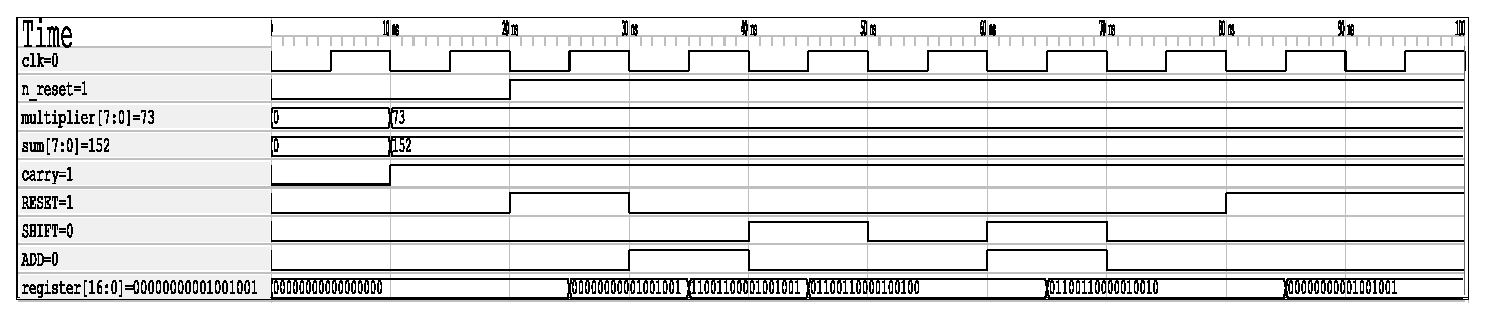
\includegraphics[scale=0.65]{../out/regs_tb.eps}
    \caption{Output waveform of the register testbench.}
    \label{fig:regstbw}
\end{figure}

The testbench for the register module as shown in listing \ref{ls:regstb} tests the register by checking its output value based on its operations on some arbitrary input values. After each stage it checks the value of the register to make sure that it is equal to the expected value.

Figure \ref{fig:regstbw} shows the resulting waveform of the testbench. As expected, despite being activated earlier, instructions are only executed on rising clock edges. This is shown as a change in the value of \lstinline{register[16:0]} in sync with a rising edge of \lstinline{clk}. For example, the multiplier is first loaded in to the register at \SI{25}{\nano\second}, at the same time as the clock edge. The changes in the register value are the same as those checked for in the testbench, showing that the register is working as expected.

\section{Sequencer design, simulation and synthesis}

\begin{figure}
    \centering
        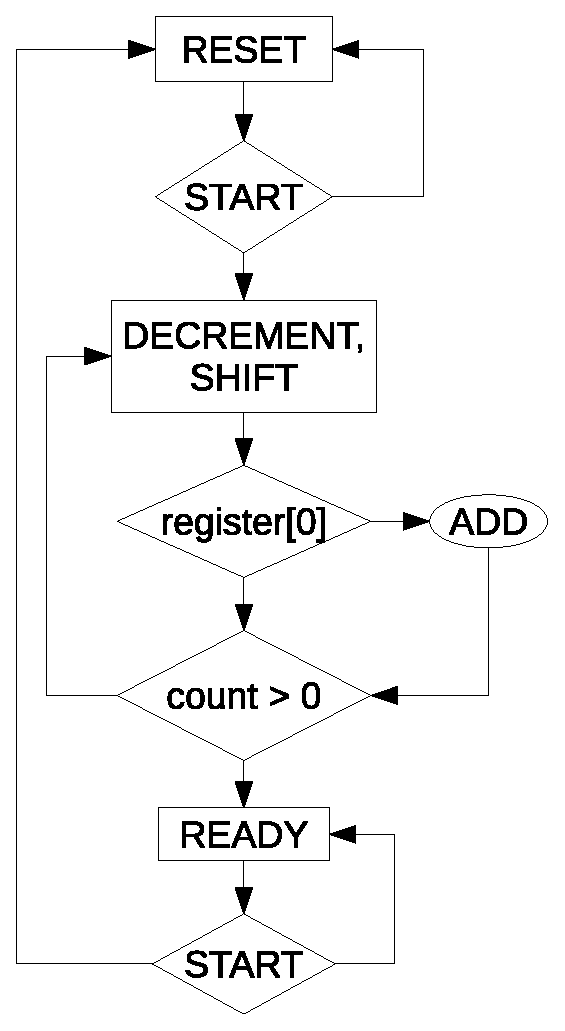
\includegraphics[scale=0.65]{finalSequencerASM.eps}
    \caption{ASM chart of the sequencer used in the final multiplier design.}
    \label{fig:fseqASM}
\end{figure}

Give the ASM chart of your sequencer and the code you developed. Explain your code and your testbench.  Give Modelsim results and Synplify RTL synthesis diagram (you may want to use advantage of the ‘state machine’ diagram drawing option in Synplify). 



\section{Multiplier design, simulation and synthesis}
If you have modified the code provided for the encapsulating module code, include it. In particular explain briefly how you handled the inputs M and Q.  Give Modelsim results and Synplify RTL synthesis diagram. 

\section{Extensions}
State if extensions were attempted. If yes, include your modified code and Modelsim results for the modified multiplier. State if your extensions worked correctly

\section{Conclusion}
State which objectives have been achieved. Give your general conclusion, what you learnt etc. Comment on ways to improve the design or extend it further  (max. 1/4 of a page).

\section{References}
Quote the sources of your information. Especially make reference to any sources you used in the development of your code. 
  
\end{document}